\documentclass[a4paper,10pt]{scrartcl}
\usepackage[utf8]{inputenc}
\usepackage{longtable}
\usepackage{amsmath}
\usepackage{amssymb}
\usepackage{textcomp}
\usepackage{listings}
\usepackage{graphicx}
\usepackage[usenames,dvipsnames,svgnames,table]{xcolor}
\usepackage{algorithm}
\usepackage{algorithmic}
\floatname{algorithm}{Algoritmo}
\renewcommand{\listalgorithmname}{Lista de algoritmos}
\renewcommand{\algorithmicrequire}{\textbf{Entrada:}}
\renewcommand{\algorithmicensure}{\textbf{Salida:}}
\renewcommand{\algorithmicend}{\textbf{fin}}
\renewcommand{\algorithmicif}{\textbf{si}}
\renewcommand{\algorithmicthen}{\textbf{entonces}}
\renewcommand{\algorithmicelse}{\textbf{en otro caso}}
\renewcommand{\algorithmicelsif}{\algorithmicelse,\ \algorithmicif}
\renewcommand{\algorithmicendif}{\algorithmicend\ \algorithmicif}
\renewcommand{\algorithmicfor}{\textbf{para }}
\renewcommand{\algorithmicforall}{\textbf{para todo}}
\renewcommand{\algorithmicdo}{\textbf{}}
\renewcommand{\algorithmicendfor}{\algorithmicend\ \algorithmicfor}
\renewcommand{\algorithmicwhile}{\textbf{mientras}}
\renewcommand{\algorithmicendwhile}{\algorithmicend\ \algorithmicwhile}
\renewcommand{\algorithmicloop}{\textbf{repetir}}
\renewcommand{\algorithmicendloop}{\algorithmicend\ \algorithmicloop}
\renewcommand{\algorithmicrepeat}{\textbf{repetir}}
\renewcommand{\algorithmicuntil}{\textbf{hasta que}}
\renewcommand{\algorithmicprint}{\textbf{imprimir}} 
\renewcommand{\algorithmicreturn}{\textbf{devolver}} 
\renewcommand{\algorithmictrue}{\textbf{true }} 
\renewcommand{\algorithmicfalse}{\textbf{false }} 
\renewcommand{\algorithmicand}{\textbf{y}} 
\renewcommand{\algorithmicor}{\textbf{o}} 

%\usepackage{pstricks,pst-node,pst-tree}
\usepackage{tikz}
\usetikzlibrary{trees}
\usepackage{tikz-qtree}

\everymath{\displaystyle}
\def\O{\mathcal{O}}
\def\hora{3,6\cdot10^{9}}
\def\dia{8,64\cdot10^{10}}
\def\semana{6,048\cdot10^{11}}
\def\anio{3,15\cdot10^{13}}
\def\anios{3,15\cdot10^{16}}
\def\Problema#1#2{\textbf{Problema #1} \textsl{#2}\\}
\def\C#1{\texttt{#1}}
\def\figurename{Figura}
\setlength{\parindent}{0cm}
%opening
\title{Reto 4: Árboles}
\author{Francisco David Charte Luque\and
        Ignacio Cordón Castillo}
\date{}

\begin{document}
\maketitle
\section{Inorden no recursivo}
        \textit{Diseñar un procedimiento inorden no recursivo a imagen y semejanza
        del procedimiento preorden no recursivo que el profesor diseñó en la clase.}\\\
 
 La idea seguida en el procedimiento de inorden iterativo es acumular en una pila
 cada elemento pendiente de mostrar, e ir descendiendo en los hijos izquierda de cada nodo
 hasta encontrar una hoja. Entonces, se imprime la hoja y se comienza a ascender
 por el árbol, mostrando los padres y entrando en los hijos derecha. Cada vez que se pasa por un
 nodo nuevo (que no se haya visitado antes), se reinicia la búsqueda en los hijos izquierda.\\\
 
 A continuación mostramos la implementación del método en C++:\\\
 
 \leftskip=1em
 \small
 \texttt{% Generator: GNU source-highlight, by Lorenzo Bettini, http://www.gnu.org/software/src-highlite
\noindent
\mbox{}\textcolor{ForestGreen}{void}\ \textbf{\textcolor{Black}{inordenNR}}\textcolor{BrickRed}{(}\textbf{\textcolor{Blue}{const}}\ ArbolBinario\textcolor{BrickRed}{\textless{}}\textcolor{ForestGreen}{int}\textcolor{BrickRed}{\textgreater{}\&}\ a\textcolor{BrickRed}{)}\textcolor{Red}{\{} \\
\mbox{}\ \ \ \ ArbolBinario\textcolor{BrickRed}{\textless{}}\textcolor{ForestGreen}{int}\textcolor{BrickRed}{\textgreater{}::}\textcolor{TealBlue}{Nodo}\ actual\textcolor{BrickRed}{;} \\
\mbox{}\ \ \ \ \textcolor{TealBlue}{stack\textless{}ArbolBinario\textless{}int\textgreater{}::Nodo\textgreater{}}\ p\textcolor{BrickRed}{;} \\
\mbox{}\ \ \ \ \textcolor{ForestGreen}{bool}\ subiendo\ \textcolor{BrickRed}{=}\ \textbf{\textcolor{Blue}{false}}\textcolor{BrickRed}{;}\ \ \ \  \\
\mbox{} \\
\mbox{}\ \ \ \ actual\textcolor{BrickRed}{=}a\textcolor{BrickRed}{.}\textbf{\textcolor{Black}{raiz}}\textcolor{BrickRed}{();} \\
\mbox{}\ \ \ \ p\textcolor{BrickRed}{.}\textbf{\textcolor{Black}{push}}\textcolor{BrickRed}{(}ArbolBinario\textcolor{BrickRed}{\textless{}}\textcolor{ForestGreen}{int}\textcolor{BrickRed}{\textgreater{}::}nodo$\_$nulo\textcolor{BrickRed}{);} \\
\mbox{}\ \ \ \ p\textcolor{BrickRed}{.}\textbf{\textcolor{Black}{push}}\textcolor{BrickRed}{(}actual\textcolor{BrickRed}{);} \\
\mbox{}\ \ \ \  \\
\mbox{}\ \ \ \ \textbf{\textcolor{Blue}{while}}\ \textcolor{BrickRed}{(}actual\ \textcolor{BrickRed}{!=}\ ArbolBinario\textcolor{BrickRed}{\textless{}}\textcolor{ForestGreen}{int}\textcolor{BrickRed}{\textgreater{}::}nodo$\_$nulo\textcolor{BrickRed}{)}\textcolor{Red}{\{} \\
\mbox{}\ \ \ \ \ \ \ \ \textbf{\textcolor{Blue}{if}}\ \textcolor{BrickRed}{(}a\textcolor{BrickRed}{.}\textbf{\textcolor{Black}{izquierda}}\textcolor{BrickRed}{(}actual\textcolor{BrickRed}{)}\ \textcolor{BrickRed}{!=}\ ArbolBinario\textcolor{BrickRed}{\textless{}}\textcolor{ForestGreen}{int}\textcolor{BrickRed}{\textgreater{}::}nodo$\_$nulo\ \textcolor{BrickRed}{\&\&}\ \textcolor{BrickRed}{!}subiendo\textcolor{BrickRed}{)}\textcolor{Red}{\{} \\
\mbox{}\ \ \ \ \ \ \ \ \ \ \ \ \textit{\textcolor{Brown}{//\ Pasamos\ a\ manejar\ el\ hijo\ izquierdo}} \\
\mbox{}\ \ \ \ \ \ \ \ \ \ \ \ actual\ \textcolor{BrickRed}{=}\ a\textcolor{BrickRed}{.}\textbf{\textcolor{Black}{izquierda}}\textcolor{BrickRed}{(}actual\textcolor{BrickRed}{);} \\
\mbox{}\ \ \ \ \ \ \ \ \ \ \ \ p\textcolor{BrickRed}{.}\textbf{\textcolor{Black}{push}}\textcolor{BrickRed}{(}actual\textcolor{BrickRed}{);} \\
\mbox{}\ \ \ \ \ \ \ \ \textcolor{Red}{\}}\ \textbf{\textcolor{Blue}{else}}\ \textcolor{Red}{\{} \\
\mbox{}\ \ \ \ \ \ \ \ \ \ \ \ cout\ \textcolor{BrickRed}{\textless{}\textless{}}\ a\textcolor{BrickRed}{.}\textbf{\textcolor{Black}{etiqueta}}\textcolor{BrickRed}{(}actual\textcolor{BrickRed}{)}\ \textcolor{BrickRed}{\textless{}\textless{}}\ \texttt{\textcolor{Red}{'\ '}}\textcolor{BrickRed}{;} \\
\mbox{}\ \ \ \ \ \ \ \ \ \ \ \ p\textcolor{BrickRed}{.}\textbf{\textcolor{Black}{pop}}\textcolor{BrickRed}{();} \\
\mbox{}\ \ \ \ \ \ \ \ \ \ \ \ subiendo\ \textcolor{BrickRed}{=}\ \textbf{\textcolor{Blue}{true}}\textcolor{BrickRed}{;} \\
\mbox{}\ \ \ \ \ \ \ \ \ \ \ \  \\
\mbox{}\ \ \ \ \ \ \ \ \ \ \ \ \textbf{\textcolor{Blue}{if}}\ \textcolor{BrickRed}{(}a\textcolor{BrickRed}{.}\textbf{\textcolor{Black}{derecha}}\textcolor{BrickRed}{(}actual\textcolor{BrickRed}{)}\ \textcolor{BrickRed}{!=}\ ArbolBinario\textcolor{BrickRed}{\textless{}}\textcolor{ForestGreen}{int}\textcolor{BrickRed}{\textgreater{}::}nodo$\_$nulo\textcolor{BrickRed}{)}\ \textcolor{Red}{\{} \\
\mbox{}\ \ \ \ \ \ \ \ \ \ \ \ \ \ \ \ \textit{\textcolor{Brown}{//\ Pasamos\ a\ manejar\ el\ hijo\ derecho}} \\
\mbox{}\ \ \ \ \ \ \ \ \ \ \ \ \ \ \ \ actual\ \textcolor{BrickRed}{=}\ a\textcolor{BrickRed}{.}\textbf{\textcolor{Black}{derecha}}\textcolor{BrickRed}{(}actual\textcolor{BrickRed}{);} \\
\mbox{}\ \ \ \ \ \ \ \ \ \ \ \ \ \ \ \ p\textcolor{BrickRed}{.}\textbf{\textcolor{Black}{push}}\textcolor{BrickRed}{(}actual\textcolor{BrickRed}{);} \\
\mbox{}\ \ \ \ \ \ \ \ \ \ \ \ \ \ \ \ subiendo\ \textcolor{BrickRed}{=}\ \textbf{\textcolor{Blue}{false}}\textcolor{BrickRed}{;} \\
\mbox{}\ \ \ \ \ \ \ \ \ \ \ \ \textcolor{Red}{\}}\ \textbf{\textcolor{Blue}{else}}\ \textcolor{Red}{\{}\  \\
\mbox{}\ \ \ \ \ \ \ \ \ \ \ \ \ \ \ \ \textit{\textcolor{Brown}{//\ Trataremos\ de\ saltar\ al\ hermano}} \\
\mbox{}\ \ \ \ \ \ \ \ \ \ \ \ \ \ \ \ actual\ \textcolor{BrickRed}{=}\ p\textcolor{BrickRed}{.}\textbf{\textcolor{Black}{top}}\textcolor{BrickRed}{();} \\
\mbox{}\ \ \ \ \ \ \ \ \ \ \ \ \textcolor{Red}{\}} \\
\mbox{}\ \ \ \ \ \ \ \ \textcolor{Red}{\}} \\
\mbox{}\ \ \ \ \textcolor{Red}{\}} \\
\mbox{}\textcolor{Red}{\}}
}
 \normalsize
 \leftskip=0em
 
 \section{Codificación de árbol binario}
         \textit{Dar un procedimiento para guardar un árbol binario en disco de forma que se
         recupere la estructura jerárquica de forma unívoca usando el mínimo número
         de centinelas que veais posible.}\\\
 
 
 El método escogido consiste en especificar, para cada nodo del árbol binario, 
 la manera en que se estructuran sus hijos. Es decir, en la codificación 
 podremos conocer si un nodo tiene dos hijos, sólo el
 izquierdo, solo el derecho o ninguno. Para ello, se recorrerá el árbol en preorden,
 añadiendo después de cada nodo, en caso de ser necesario, uno
 de los tres centinelas siguientes:
  
 \begin{enumerate}
 \item[i.] \texttt{<} Le falta el hijo izquierdo
 \item[ii.] \texttt{>} Le falta el hijo derecho
 \item[iii.] \texttt{-} No tiene hijos
 \end{enumerate}
 
 No se hará empleo de ningún centinela si el nodo tiene ambos hijos,
 ni tampoco tendrá centinela el último nodo, pues este 
 siempre será \texttt{-}. Veamos un ejemplo: para el árbol siguiente
 
 \begin{center}
 \begin{minipage}{20pt}
 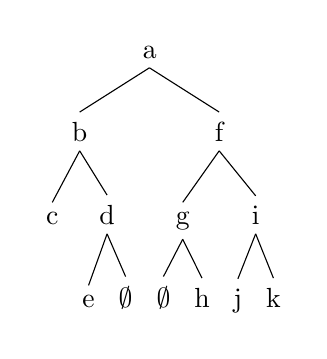
\begin{tikzpicture}
 \node{\Tree 
  [.{a} 
     [.b
         [.c ]
         [.d e $\emptyset$ ] ]
     [.f
         [.g $\emptyset$ h ]
         [.i j k ] ]
  ]};\\
 \end{tikzpicture}
 \end{minipage}
 \end{center}
 
 se obtendrá la codificación \texttt{abc-d>e-fg<h-ij-k}.\\\ %ajustar ejemplo a posición de centinelas \texttt{ab-c>d-ef<g-hi-j-k}
 
 Para esta codificación, se tiene que en el peor caso posible para
 $n$ nodos(aquel en que a cada nodo le falta un hijo, y por tanto cada nodo va acompañado
 de un centinela), se usan $n-1$ centinelas; esto es, se tiene que se
 emplean $2n-1$ posiciones (entre centinelas y etiquetas). 
 El siguiente árbol ilustra este caso, tomando todos los nodos distintos de la raíz como
 hijos izquierdos del padre:\\
 
 \begin{center}
 \begin{minipage}{20pt}
    \begin{tikzpicture}
 \node{\Tree 
  [.a
    [.b
        [.c
           [.d 
            \edge[dashed] {};
            [.n ]]]]
  ]};\\
 \end{tikzpicture}
 \end{minipage}
 \end{center}
 
 La codificación resultante del árbol sería: \texttt{a>b>c>d>\ldots n}.\\\
 
 El procedimiento se ha desarrollado en dos partes: la primera ejecuta una
 preparación de los datos, para un manejo recursivo por la segunda. Es conveniente
 aclarar que algoritmo \ref{rec2} trabaja directamente con los
 datos, no con una copia, es decir, está modificando en cada ejecución
 el árbol \texttt{nuevo} y las pilas \texttt{hijos} y \texttt{nodos} que se pasan 
 desde el algoritmo \ref{rec1}. Además, para evitar añadir complejidad
 innecesaria a la descripción de los algoritmos, se han identificado los
 tipos de dato del nodo del árbol y el de la etiqueta (se realizan asignaciones
 de etiquetas a nodos).
  
 % Aclarar que se identifica el tipo nodo con el tipo etiqueta...
  
      \begin{algorithm}[H]
      \begin{algorithmic}[1]
     \REQUIRE \ \\
         \texttt{bin\_tree}, árbol binario leído codificado\\\
     
     \STATE{Crear pila \texttt{nodos}, 
            pila \texttt{hijos}}
     \STATE{\texttt{centinelas $\gets$ \{-,<,>\}}}
     \\\
     \FORALL{\texttt{elemento} $en$ \texttt{bin\_tree}}
       \IF{\texttt{elemento} $\in$ \texttt{centinelas}}
         \STATE{Apilar \texttt{elemento} en \texttt{hijos}}
       \ELSE
         \STATE{Apilar \texttt{elemento} en \texttt{nodos}}
         \IF{$\nexists$ posterior a \texttt{elemento} \OR posterior a \texttt{elemento} $\notin$ \texttt{centinelas}}
           \STATE{Apilar * en \texttt{hijos}}
         \ENDIF
       \ENDIF
     \ENDFOR
     %\STATE{Apilar último elemento $en$ \texttt{bin\_tree} en \texttt{nodos}}
     \STATE{Apilar \texttt{-} en \texttt{hijos}}
     \\\
     \STATE{Crear árbol \texttt{nuevo}}
     \STATE{Raíz de \texttt{nuevo} $\gets$ tope de \texttt{nodos}}
     \STATE{Sacar tope de \texttt{nodos}}
     \STATE{Llamar al algoritmo \ref{rec2} con parámetros \{raíz de \texttt{nodos}, \texttt{nodos}, \texttt{hijos}\}}
     \\\
     \RETURN \texttt{nuevo}
      \end{algorithmic}
      \caption{Recuperación del árbol (I)}
      \label{rec1}
      \end{algorithm}
   
      \begin{algorithm}[H]
      \begin{algorithmic}[1]
     \REQUIRE \ \\
         \texttt{actual}, nodo sobre el que añadir descendientes\\
         \texttt{nodos}, pila de nodos\\
         \texttt{hijos}, pila de centinelas\\\  
     
     \STATE \texttt{centinela} $\gets$ tope de \texttt{hijos}
     \STATE{Sacar tope de \texttt{hijos}}
     \IF{\texttt{centinela} $\neq$ \texttt{-}}
     \IF{\texttt{centinela} $\neq$ \texttt{<}}
         \STATE{Hijo izquierda de \texttt{actual}
                $\gets$ tope de \texttt{nodos}}
         \STATE{Sacar tope de \texttt{nodos}}
         \STATE{Llamar al algoritmo \ref{rec2} con parámetros
               \{hijo izquierda de \texttt{actual}, \texttt{nodos}, \texttt{hijos}\}}
     \ENDIF
     \\\
     \IF{\texttt{centinela} $\neq$ \texttt{>}}
       \STATE{Hijo derecha de \texttt{actual}
               $\gets$ tope de \texttt{nodos}}
        \STATE{Sacar tope de \texttt{nodos}}
       \STATE{Llamar al algoritmo \ref{rec2} con parámetros 
             \{hijo derecha de \texttt{actual}, \texttt{nodos}, \texttt{hijos}\}}
     \ENDIF
     \ENDIF
      \end{algorithmic}
      \caption{Recuperación del árbol (II)}
      \label{rec2}
      \end{algorithm}
\end{document}
